\section{进动与流体}
\begin{definition}[进动]
    \textbf{进动}是指刚体绕轴旋转时，旋转轴绕另外一个轴旋转的回转现象，如图\ref{pic:3.5-1}所示.
\end{definition}
\begin{figure}[hb]
    \begin{center}
        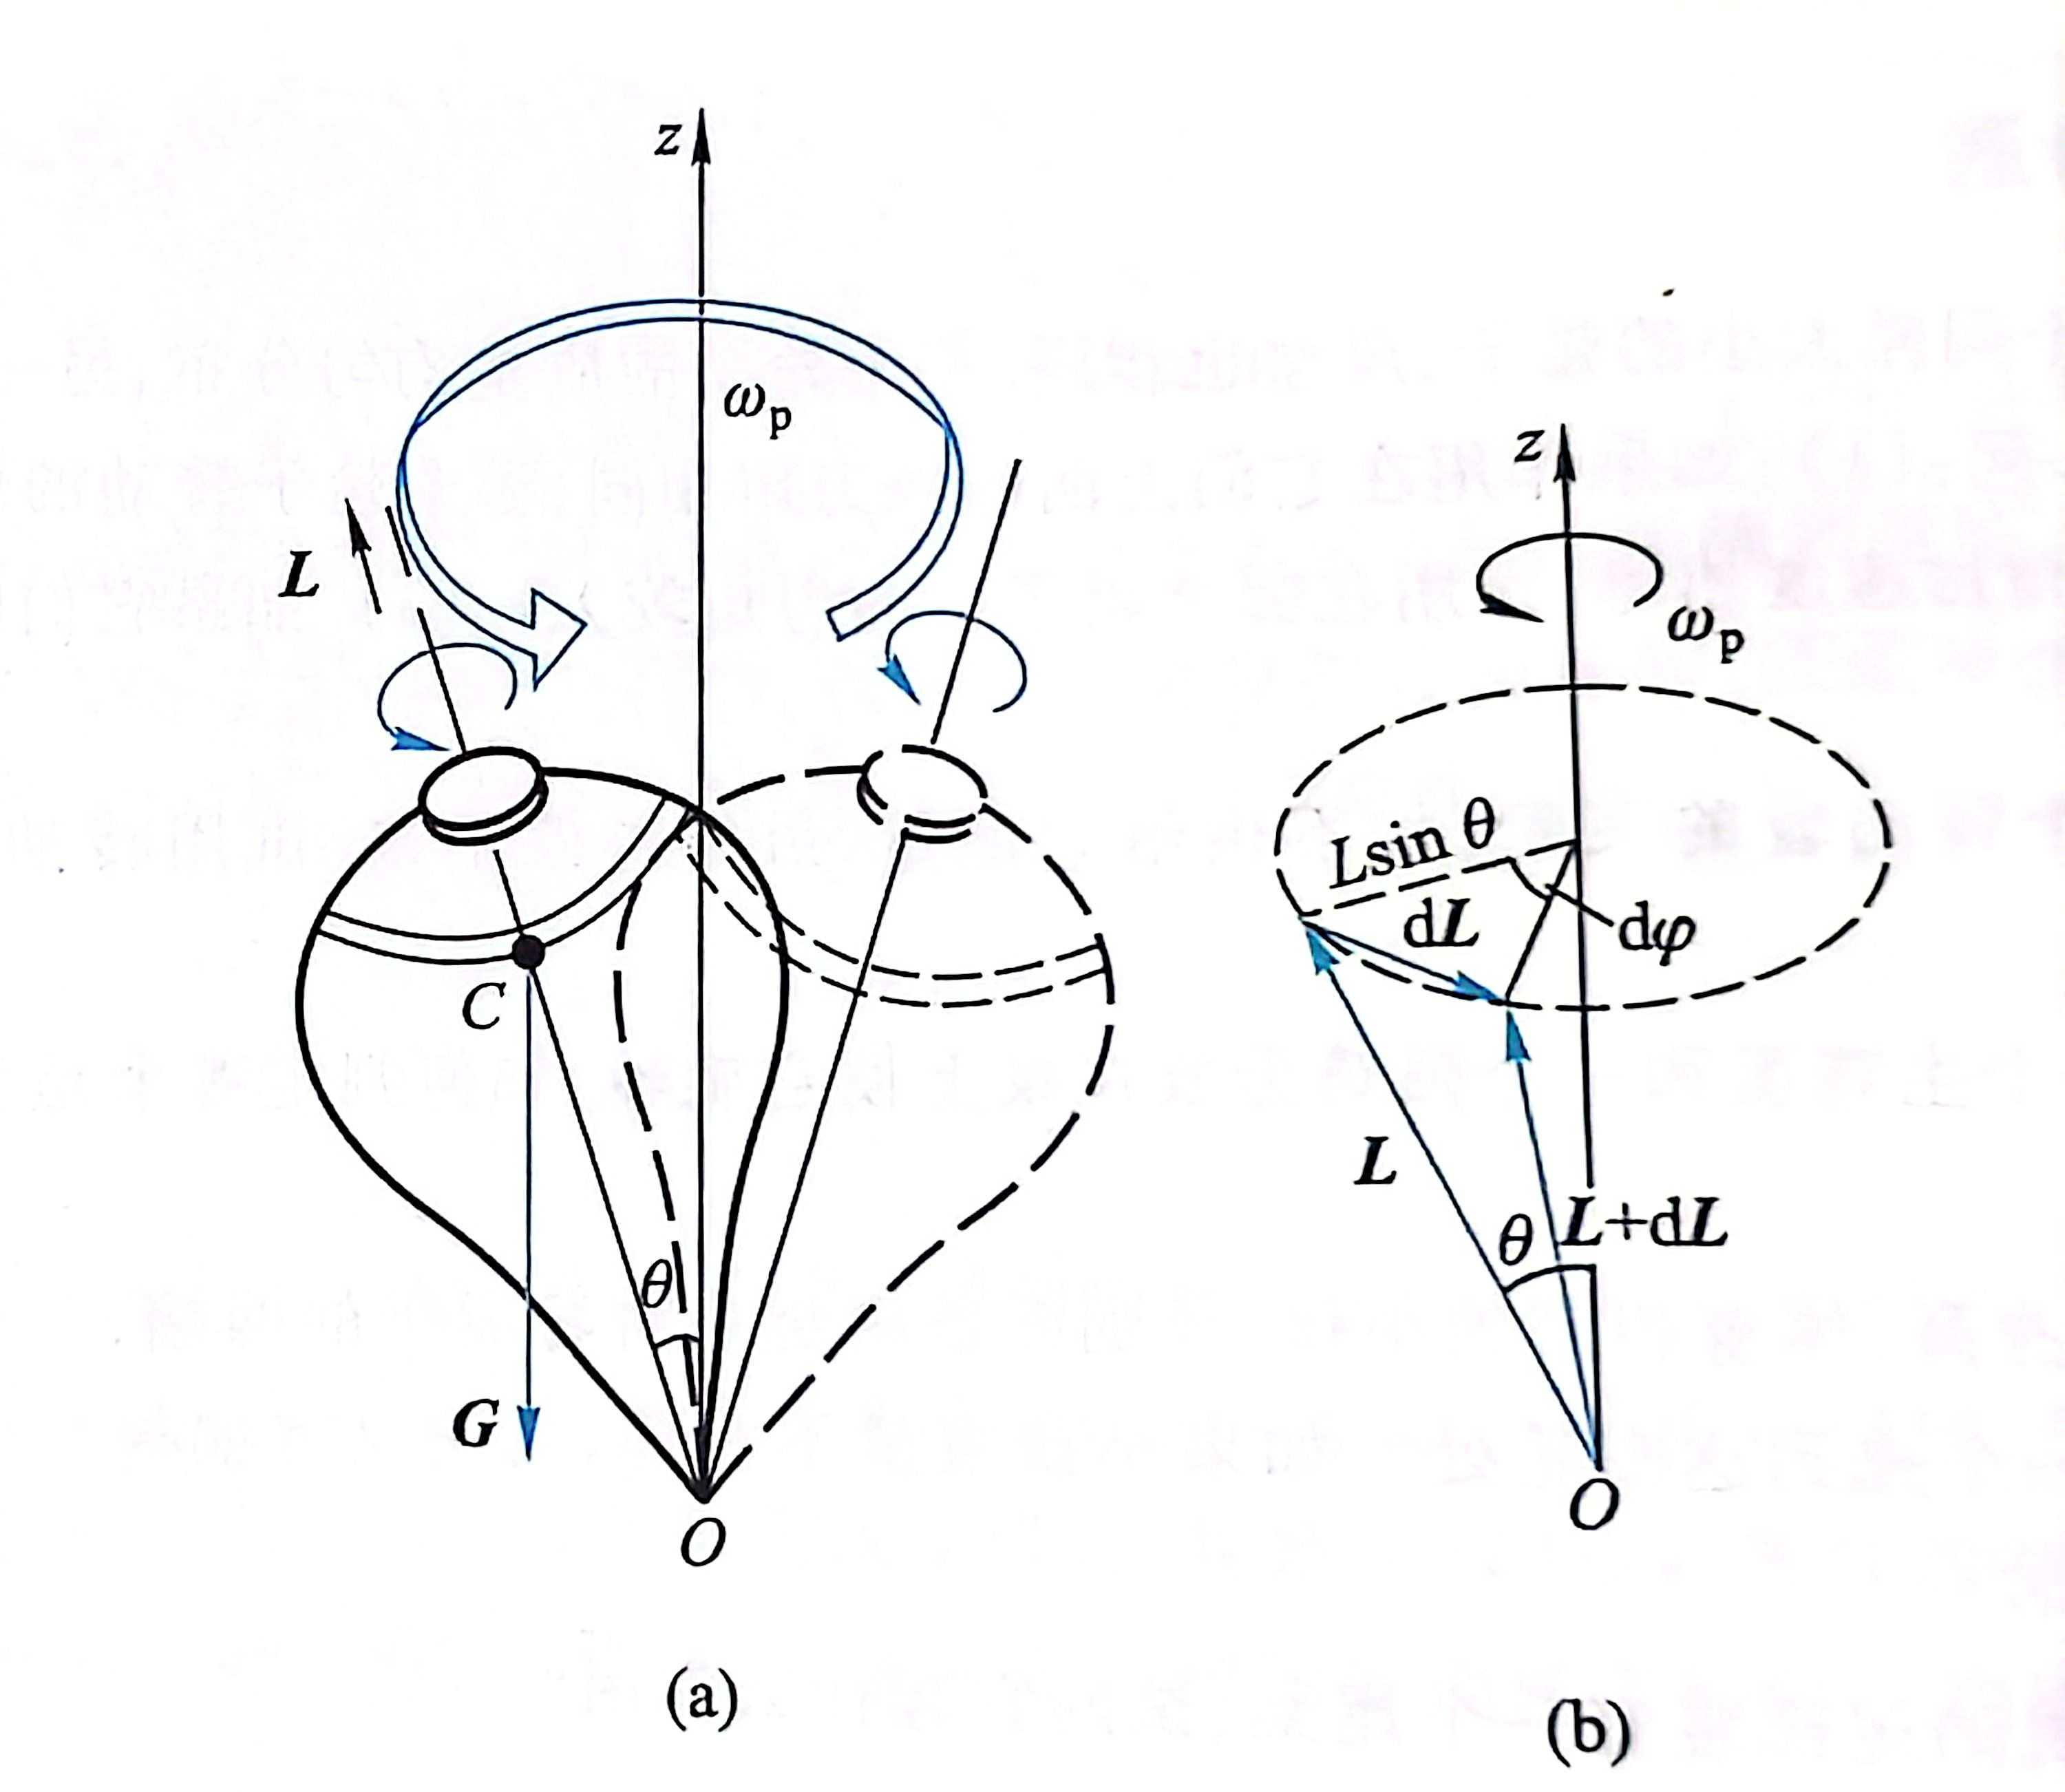
\includegraphics[width=0.6\textwidth]{images/3-5-1.jpg}
        \caption{进动示意图}
        \label{pic:3.5-1}
    \end{center}
\end{figure}

进动是由作用在刚体上与旋转轴垂直的外力矩引起的，一般出现在自转角速度较大的情况下.进动角速度可由公式\ref{equ:3.5-1}确定.

\begin{equation}
    \omega_p=\dfrac{M}{J\omega \sin\theta}
    \label{equ:3.5-1}
\end{equation}

在自转角速度较小的情况下，刚体可能还会\textbf{章动}，在此不详细介绍.

\begin{definition}[定常流动]
    流场中各点流速不随时间变化的流动称为\textbf{定常流动}.
\end{definition}

对于不可压缩，没有黏性的\textbf{理想流体}，有伯努利方程，表明作定常流动的流体中，在同一流管中任何一点处，流体每单位体积的动能和势能以及在该处的压强之和为常量.在工程中，该方程常表示为公式\ref{equ:3.5-2}.
\begin{equation}
    \dfrac{p}{\rho g}+\dfrac{v^2}{2g}+h=Const
    \label{equ:3.5-2}
\end{equation}
其中，公式\ref{equ:3.5-2}左端各项依次称为压力头（表征压力）、速度头（表征动能）、水头（表征势能），公式右端表示一个（具有长度量纲的）常数.